\chapter{Introduction}


Test af skrift type \\
Prøve: \cite{example} Test

\section{Background}
\subsection{Technology}
\subsection{The Danish Healthcare System}



The establishment of the Danish Healthcare System started in the eighteenth century. The first hospital was placed in Copenhagen and it opened in 1757. This hospital is still functioning and is today known as Rigshospitalet. Outside the capital small hospitals were build during the late eighteenth century. Even then the hospital was partly financed by taxes, patient payment and charity. In the late nineteenth century every thirteenth Dane was a member in a sick-benefit association which the Danish Government co-funded. The Danish Welfare State has its root in 1933 where the Social reform was founded. With this reform Danes with a low income it became a demand that they were members of a sick.benefit association. During the thirties taxes gradually became the dominant finance source to the Danish Healthcare System.\\ 
The sick-benefit associations was shut down in 1973 and replaced by public health insurance. The Danish public health insurance is paid by the Danes themselves within taxes. But the insurance provides free care for everyone regardless of  income and residence. This public health insurance includes hospital stays, surgery, visits to a GP and specialist'. Furthermore it provides partly funding for dentist, physiotherapist, chiropractor, podiatrist and contributes to medicin.   \\
Every healthcare system consist of users, healthcare institutions and the financial third part, besides the fundamental financial mechanism user fee, tax and budgets/rates. This is described with the tripartite model in \cref{Trepartmodel}. The A, B and C is the financial mechanism and 1, 2 and 3 is the consistence of the healthcare system. The model shows how a third part is pushed in between the users and the healthcare institutions. This third part creates equality between users as much as possible. The constellation of finances differs from country to country. Denmark is mostly funded by the Government through taxes whereas US citizen needs health insurance to pay the for these services. \\
 

\begin{figure}[H]
\centering
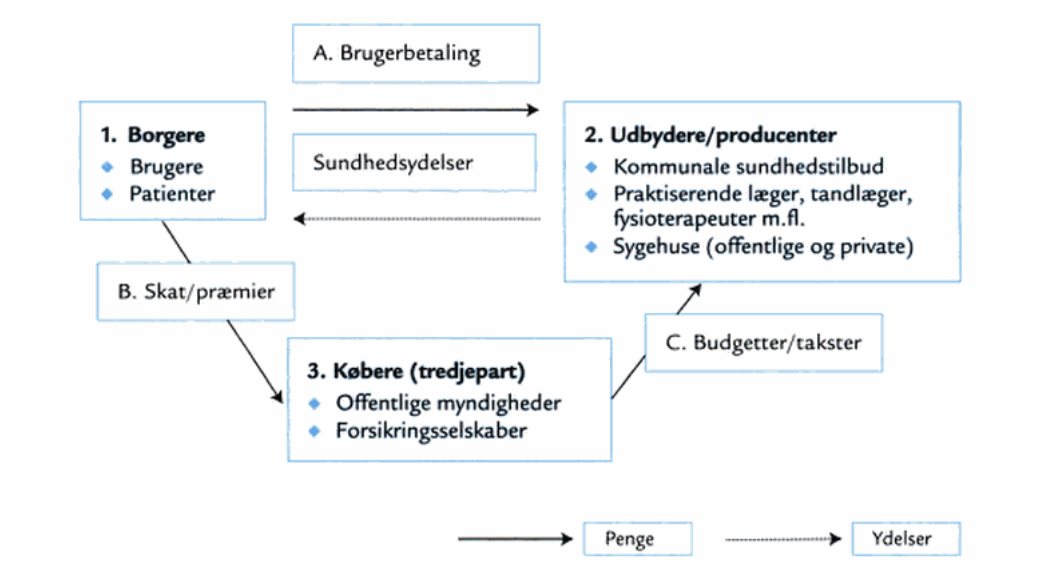
\includegraphics[width=1\textwidth]{Figure/tredjepart.png}
\caption{Tripartite model \cite{sundhedsvaesen}}
\label{Trepartmodel}
\end{figure} 

In 2007 Denmark made big structural changes throughout the healthcare organisation. Municipalities was combined which meant a change from 275 municipalities to 98. The 14 counties was replaced with by 5 regions. The Danish Healthcare System is thereby organized in three levels: State, region and municipalities.

 in 1927 there was a total of 160 somatic hospitals in Denmark. 



omlægning fra amt til regioner
\cite{sundhedsvaesen}
\subsection{Target Group and Market Segment}


\section{Problemstatement}
The total cost of treating cardiovascular patients at the hospitals in Denmark was 5.5 billion DKK in 2015. The incidence is approximately 55.700 a year. About 107.100 Danes get admitted to the hospital every year due to a cardiovascular disease. Overall this will be 148.600 admission due to approximately 23 percent of the cardiovascular patients are readmitted into the hospital within 30 days after being discharged. Beyond the admissions the Danish system have 73.100 ambulant consultation within the hospital. Every year 12.400 Danish citizens dies from cardiovascular disease and it is thereby the second most common cause of death in Denmark . 

All this indicates that cardiovascular patients constitute a large part of the Danish states economy. This leads to our problem statement which is:

•	How can ICT be used to shorten hospital stay for cardiovascular patients?
•	Which barriers/challenges can such system meet in implementation?
•	What impact would an ICT solution for rehabilitation have on both cardiovascular patients and the Danish healthcare system?


\subsection{Delimitation}
      

